\documentclass[a4paper,12pt,oneside]{report}

\usepackage{fancyhdr}
\usepackage[magyar]{babel}
\usepackage{t1enc}
\usepackage[utf8]{inputenc}
\usepackage{graphicx}
\usepackage{todonotes}
\usepackage[section,numbib,nottoc]{tocbibind}
\usepackage{hyperref}
\usepackage{amssymb}
\usepackage{booktabs}
\usepackage{pdflscape}
\usepackage{formai_kovetelmenyek}

\usepackage{array} % for defining a new column type
\usepackage{varwidth} %for the varwidth minipage environment

\usepackage{usecases} %usecasehez

\hypersetup{
    pdfauthor={Varga Marcell},
    pdftitle={Képfeldolgozást támogató keretrendszer és modulok készítése}
}

\lstset{
     basicstyle = \ttfamily\footnotesize
    ,breaklines = true
    ,prebreak   = \raisebox{0ex}[0ex][0ex]{\ensuremath{\hookleftarrow}}
    ,extendedchars = true
    ,literate={á}{{\'a}}1 {ó}{{\'o}}1 {é}{{\'e}}1 {í}{{\'i}}1 {ő}{{\~o}}1 {ö}{{\"o}}1 {ű}{{\'u}}1
}

\hyphenation{Google}

\title{Képfeldolgozást támogató keretrendszer és modulok készítése}
\author{Varga Marcell}
\date{}

%fattyú- és árvasorok büntetése, ha nagyobb, akkor jobban próbálja elkerülni
\widowpenalty=400
\clubpenalty=400

\graphicspath{{./kepek/}}

\setcounter{secnumdepth}{3} %szamozza a subsubsection-oket is
\AtBeginDocument{\addtocontents{toc}{\protect\pagestyle{empty}}} %ezzel erem el, hogy a tartalomjegyzek ne kapjon oldalszamot
\AtBeginDocument{\addtocontents{tod}{\protect\thispagestyle{empty}}}

\begin{document}
\newcolumntype{M}{>{\begin{varwidth}{4cm}}l<{\end{varwidth}}} %M is for Maximal column

\setcounter{chapter}{1}

\pagestyle{empty}
%------------------------------------------------------------------
% külsõ kötéstábla
{
    \begin{center}
    \vspace*{5cm}
    {
        \Huge SZAKDOLGOZAT}\\
        \vspace*{10cm}
        {\LARGE Varga Marcell}\\
        \vspace*{3cm}
        {\LARGE 2014}
    \end{center}
}
\newpage

% címoldal
\begin{center}
{
    \Large Pannon Egyetem\\
    Matematika Tanszék\vspace*{3mm}\\
    Mérnök informatikus BSc szak
}
    \vspace*{2cm}\\
    {\LARGE \bf SZAKDOLGOZAT}
    \vspace{3cm}\\
    {\LARGE\bf Képfeldolgozást támogató keretrendszer és modulok készítése}
    \vspace{3cm}\\
    {\large Varga Marcell}
    \vspace{6cm}
    \\
    {\large Témavezető: Lipovits Ágnes}
    \vspace{1cm}\\
    {\large 2014}
\end{center}
\normalsize
% címlap vége
\newpage

Ide jön az eredeti vagy a fénymásolt feladatkiírás.
\newpage

\begin{center}
\section*{Nyilatkozat}
\end{center}

Alulírott Varga Marcell diplomázó hallgató kijelentem, hogy a szakdolgozatot a Pannon Egyetem Matematika Tanszékén készítettem Mérnök informatikus BSc szak (BSc in Computer Engineering
) megszerzése érdekében.

Kijelentem, hogy a szakdolgozatban lévő érdemi rész saját munkám eredménye, az érdemi részen kívül csak a hivatkozott forrásokat (szakirodalom, eszközök, stb.) használtam fel.

Tudomásul veszem, hogy a szakdolgozatban foglalt eredményeket a Pannon Egyetem, valamint a feladatot kiíró szervezeti egység saját céljaira szabadon felhasználhatja.\\

\begin{flushleft}
{Veszprém, 2014. május 02.\\}
\end{flushleft}

\begin{flushright}
{Aláírás \vspace{4cm}}
\end{flushright}

Alulírott Lipovits Ágnes témavezető kijelentem, hogy a szakdolgozatot Varga Marcell a Pannon Egyetem Matematika Tanszékén készítette Mérnök informatikus BSc szak (BSc in Computer Engineering) megszerzése érdekében.

Kijelentem, hogy a szakdolgozat védésre bocsátását engedélyezem.\\

\begin{flushleft}
{Veszprém, 2014. május 02.\\}
\end{flushleft}

\begin{flushright}
{Aláírás}
\end{flushright}
%A tartalomjegyzék:
\newpage
\pagebreak
\begin{center}
\section*{Köszönetnyilvánítás}
\end{center}

Köszönet!
%Köszönöm a családomnak a sok türelmet és segítséget, amit kaptam, nélkülük ez a szakdolgozat nem készült volna el.
\\
\\
%Köszönöm témavezetőmnek, Lipovits Ágnes az elmúlt egy év során adott iránymutatását.
\\
\\
%Végül, de nem utolsó sorban, szeretném megköszönni a szaktársaimnak a bíztatást.

\newpage

\begin{center}
\section*{\textbf{\Large \MakeUppercase{Tartalmi összefoglaló}}}
\end{center}

E szakdolgozat témája ...

\vspace{2cm}

{\bf Kulcsszavak:} {\it szoftverarchitektúra, képfeldolgozás, adatszerkezetek, adatkezelés, Qt, c++, OpenCV}
\newpage

\newpage

\begin{center}
\section*{\textbf{\Large \MakeUppercase{Abstract}}}
\end{center}

The topic of this thesis is to ...

\vspace{2cm}

{\bf Keywords:} {\it software-architecture, image processing, data structure, data processing, Qt, c++, OpenCV}
\newpage
%--------------%------------------------------------------------------------------
\pagenumbering{gobble} %ne legyen oldalszamozas a tartalomjegyzek oldalon
\listoftodos

\renewcommand{\thefigure}{\arabic{figure}}

\setcounter{tocdepth}{3} %subsubsection-ok is latszodjanak
\thispagestyle{empty}
\tableofcontents
\pagebreak

\pagenumbering{arabic} %legyen oldalszamozas
\setcounter{page}{1} %innentől indul az oldalszámozás
\pagestyle{plain}
\fancyhead[C]{\rightmark}
\fancyfoot[R]{\thepage}

\section{A feladat összefoglalása}

Témám egy olyan képfeldolgozást támogató keretrendszer tervezése és fejlesztése, amely alkalmas képek egyedi vizsgálatára és kötegelt feldolgozásra. A feldolgozást végző algoritmusok a dinamikusan betölthető modulokban foglalnak helyet.

A rendszer fő haszonélvezője a Pannon Egyetem Képfeldolgozás Kutatólaboratóriuma lesz, de célom, hogy kellően általános rendszer jöjjön létre amelyet bárki könnyen és egyszerűen használhat, illetve bővítheti saját modulokkal.

\section{Hasonló célú rendszerek}
Munkám első részeként megvizsgáltam, hogy milyen hasonló célú szoftverek, illetve szoftver csomagok találhatóak a piacon. Erre azért volt szükség, hogy pontosabb képet kapjak a jelenleg fellelhető megoldásokról, és munkám során az így tapasztalt pozitív és negatív tapasztalatokat felhasználva jó minőségű szoftvert fejleszthessek.\\
Különböző összehasonlítási szempontokat állítottam fel, melyek lentebb olvashatóak. Az összehasonlítás során a személyes benyomáson túl, külsős véleményeket is megtekíntettem (legyen az a kiadó cégnek az ajánlása, vagy független publikáció, újságcikk).
\subsection{Összehasonlítási szempontok}

\subsubsection{Általános tulajdonságok:}
\begin{description}
	\itemsep0em
	\item Platform: Milyen környezetben és operációs rendszeren használható? Milyen program nyelvvel fejlesztették?
	\item Licence: Milyen licenc alatt került publikálásra?
	\item Cél csoport: A szoftver kinek az igényeinek teljesítésére törekszik?
	\item Támogató: Van hivatalos támogatottságga? (cég, alapítvány)
	\item Felhasználói közösség: Fórum, levelező listák?
	\item Plugin rendszer: Plugin betöltésre van lehetőségünk? Saját plugin?
	\item Kötegelt feldolgozási lehetőség: Feldolgozhatunk egyszerre nagy mennyiségű képet?
	\item Automatizálási lehetőségek: Automatizálhatjuk a feldolgozást? pl.: makrók
	\item Fejlesztői eszközök: Rendelkezik hivatalos fejlesztői eszközökkel?
	\item Támogatott bemeneti formátumok köre
	\item Megjelenítési, vizualizációs lehetőségek listája

\end{description}


\subsubsection{Képfeldolgozási képességek}
\begin{itemize}
	\itemsep0em
	\item Képjavító eljárások, pl.: élesítés, kontrasztkiegyenlítés
	\item Geometriai műveletek, pl.: átméretezés, forgatás, tükrözés
	\item Analizálás, pl.: eltérések detektálása, alacsony szintű képleírók
	\item Szerkesztési műveletek, pl.: logikai, szöveg, alakzatok elhelyezése
	\item Színterek közötti konverzió, pl.: RGB $\rightarrow $ HSL, csatornák külön kezelése stb

\end{itemize}

\subsection{Választott szoftverek}
\begin{itemize}

    \item \emph{ImageJ}\cite{website:imagej}\\
    Képfeldolgozást és analizálást végző rendszer, amely a National Institutes of Health fejlesztése.
	A program első indulásakor látható, hogy itt egy professzionális orvostechnológiai eszközről van szó.
	Támogatottsága jelentős mind közösségi, mind bővíthetőségi szempontból. Fegyvertárában olyan eszközöket is felvonultat mint Z és T funkciók.\cite{article:imagej_article}\\A Z funkciók segítségével pl.: MRI-vel készített sorozatos metszeti képeket kezelhetünk könnyedén, lehetőségeinket tovább növeli, hogy térbeli szervezés mellett még időbeli struktúra felépítésére és kezelésére is lehetőséget ad a program (T funkciók).
    
    \item \emph{ImBatch}\cite{website:imbatch}\\
    Képfeldolgozást végző rendszer. Célcsoportja a egyértelműen egy félprofesszionális felhasználói szint. Tehát itt eleve nem is várunk professzionális analitikai funkciókat. Cserébe kapunk egy szép, letisztult, egyszerű grafikus felhasználói felületet, és egy pár használatot segítő funkciót: pl.: Windows helyérzékeny menü intergrációt.
    
    \item \emph{OriginLab - Image Processing}\cite{website:originlab}\\
	Az OriginLab szoftver csomag része, amely első sorban tudományos és ipari célközöséget szolgál ki. \cite{website:originlab_about} A korábban tárgyalt rendszerekkel ellentétben ez a szoftver fizetős (21 napos teszt verzió igényelhető). Ára hozza az iparban szokásos szoftver árakat \cite{website:originlab_usd}, amely személyes felhasználásra kissé borsos, azonban funkcionalitása kárpótolja a felhasználót. Rentgeteg elemzési lehetőség mellett még OriginC-ben saját algoritmusainkat is megvalósíthatunk, a LabView támogatás már majdnem, hogy csak hab a tortán.\\
\end{itemize}
	

\subsection{Összefoglalás}
A részletes összehasonlítás a \ref{table:diff_soft}. táblázatból olvasható ki a \pageref{table:diff_soft}. oldalon.\\
Az adatsorokból megállapíthatjuk, hogy a fejleszteni kívánt szoftverünkkel szemben több fontos követelmény és megállaptás is felírható:
\begin{itemize}
	\itemsep0em
	\item Hordozható legyen több platformra. Hiszen egy laboratóriumban több féle architektúra elő fordul. (Ideális esetben tehát a szoftverünk legyen crossplatform.)
	\item Nyitott legyen a további fejlesztésekre. Hiszen az csak utópisztikus álom, hogy egyszer valaki elkészíti az funkciót és onnantól mindenki boldogan használja őket a világ végezetéig... Röviden a felhasználónak adjuk meg a lehetőséget, hogy testre szabja a szoftverünket, vagy dinamikusan külön modulokkal, pluginekkel bővíthesse azt.
	\item A célcsoport kiválasztása alapvetően meghatározza a beépített funktciókat és a felhasználói interfészt. Ha több nézetet tervezünk a programba a célközönséget szélesíthetjük.
	\item Szerepeljenek automatizálási lehetőségek. Senki nem fog egyesével nem hogy 50.000 de még 500 képet sem feldolgozni.
	\item A szoftvert gyakorlatilag bármilyen bemeneti formátum kezelésére fel kell készíteni.
	\item Már gyárilag nagy mennyiségű képjavító, feldolgozó, szerkesztő, elemző és analizáló funkcionalitással érkezzen a szoftver.

\end{itemize}

Összegezve láthatjuk, hogy eléggé könnyen lehet már előkészített rendszereket választani a szoftverpiac palettájáról. Ilyenkor jogosan felmerül a kérdés, hogy ez a projekt miben ad többet, mint a jelenlegi lehetőségek? \\
Célom, hogy egy egyszerű felhasználó számára is könnyen kezelhető nyitott bővíthető rendszer hozzak létre, ahol többszintű képfeldolgozást is egyszerűen végezhetjük. Egy blokkos jellegű grafikus felületet készíteni (mint pl.: Labview blockdiagrammjai \cite{website:ni_blocks}, vagy UDK4 BluePrint Editorja\cite{website:udk_blueprint}).

\section{Rendszertervek}
A rendszer tervezését több fő folyamatra osztottam:
\begin{enumerate}
	\itemsep0em
	\item Követelményrendszer felírása (funkcionális és nem funkcionális követelmények)
	\item Megfelelő technológiák kiválasztása követelményrendszer és egyéb szempontok alapján
	\item Alap rendszerarchitektúra elkészítése (modulok megtervezése)
	\item Felület tervek
\end{enumerate}

\subsection{Szószedet}
A tervezési munka során természetesen szükségessé vált több különböző objektum, folyamat deffiniálása és elenevezése.
A szószedet \ref{table:szoszedet}. táblázatban található a \pageref{table:diff_soft}. oldalon.

\subsection{Követelmény analízis}
A követelmény analízist a RUP (Rational Unified Process) metodika FURPS+ rendszere alapján végeztem.\\Így minden olyan tulajdonság és jellemző feltüntetésre került amely szükséges, hogy a szoftver megoldja az adott problémát. \cite{website:soft_req_def} Ezek a követelmények jellemzőjüket tekíntve lehetnek funkcionális követelmények, és nem funkcionális követelmények.

\subsubsection{Funkcionális követelmények}
Funkcionális követelményeknek tekíntünk minden olyan követelményt, amely a fő termékünkbe valamilyen képességet biztosít. pl.: Adott objektum megjelenítése \cite{website:soft_func_req_ibm}

A \ref{fig:bimg_usecase_schema}. ábrán megfigyelhető a sematikus usecase diagrammja. (A teljes diagramm a \ref{fig:bimg_usecase_schema_part_1}. ábrán és a \ref{fig:bimg_usecase_schema_part_2}. ábrán tekínthető meg a \pageref{fig:bimg_usecase_schema_part_1}. oldalon.
\begin{figure}[h]
  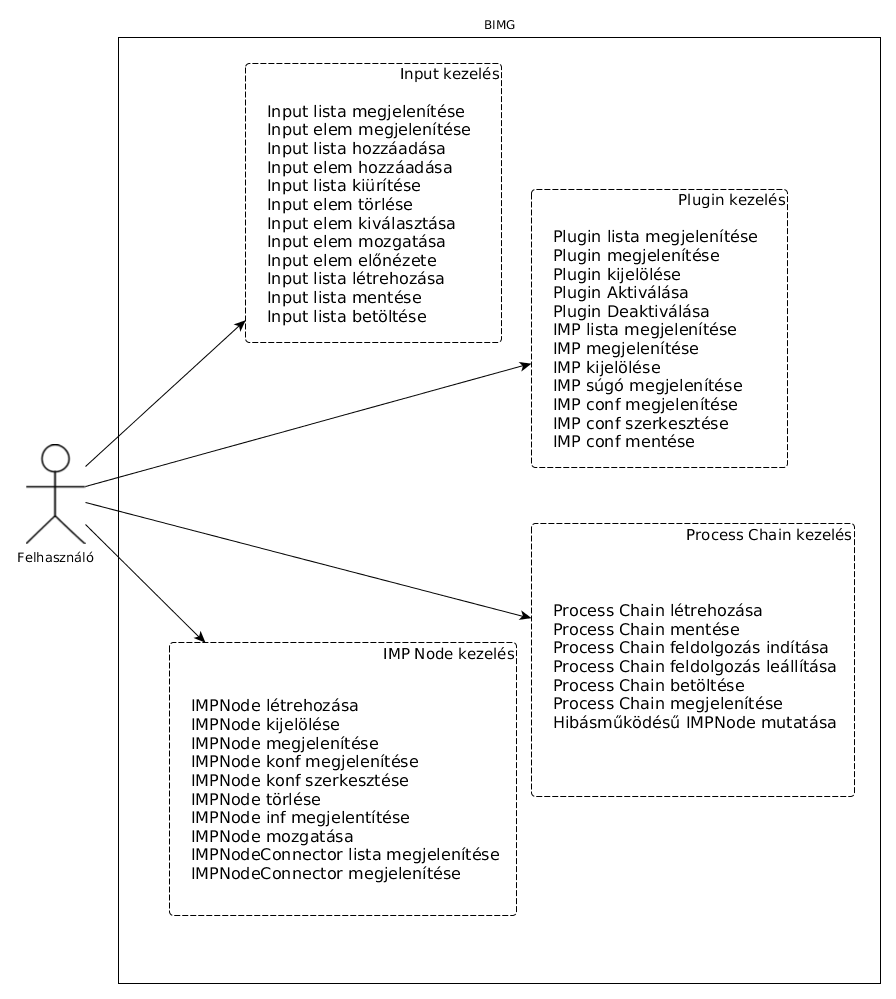
\includegraphics[width=\textwidth]{schematic_usecase.png}
  \caption{A BIMG sematikus usecase diagrammja}
  \label{fig:bimg_usecase_schema}
\end{figure}

Az egy logikai csoportba tartozó funkciókat csoportokba szerveztem. Így a következő csoportok kerültek felírásra:
\begin{itemize}
	\itemsep0em
	\item Input kezelés: itt történik az input hozzáadása, törlése, szerkesztése, az input elemek sorrendjének megváltoztatása, továbbá a bemeneti elemek megjelenítése.
	\item Plugin kezelés: itt történik a pluginek a rendszerbe töltése, ki/be kapcsolása, és tartlamuk böngészése is.
	\item Process Chain kezelés: a feldolgozás szíve, ez a modul veszi át az input listát, és végzi a feldolgozást
	\item IMP Node kezelés: Itt történik a Process Chain elemeinek a deffiniálása és az elemek közötti relációknak a beállítása.
\end{itemize}
Ezek a logikai csoportok reprezentálnak egyben egy modult is a rendszerben.
\todo{USECASE}
A teljes usecase kifejtve a mellékletben olvasható.

\subsubsection{Nem funkcionális követelmények}


\subsection{Választott technológiák}
A megfelelő technológiák kiválasztása során több tényező is befolyásolta a döntésemet. Ezekeből két nagy csoportot írtam fel: követelményrendszerből illetve szubjektív nézőpontból kiemelt fontosságú tényezők. A követelményrendszerből adódóakat a korábbi két alpontban bőségesen részleteztem, ezért a következőkben csak a szubjektív pontokat vázolnám fel.
\begin{itemize}
	\itemsep0em
	\item Egyszerű és gyors, minőségi fejlesztés
	\item Könnyű dokumentálhatóság
	\item Legyen korábbi munkáimból rutinom az adott technológiák alkalmazásában
	\item Képfeldolgozási függvénykönyvtárakkal legyenek jól ellátottak a kiválasztott technológiák (nem szeretném újra feltalálni a kereket)

\end{itemize}
A fenti szempontokból a következő fegyvertár került összeállításra:\\ A program alap szerkezete Qt-val, a képfeldolgozásért felelős komponensek OpenCv-vel kerültek megvalósításra. A verziókövetést Git-el végeztem, a dokumentáció és dolgozat elkészítéséhez pedig Latex-et, Gummi-t, és Yed-et használtam.
\subsubsection{Qt}
Egyike a legmeghatározóbb multiplatform c++-ra épülő alkalmazás keretrendszerenek. \cite{website:qt_about} Korábban már több másik projektben is sikeresen dolgoztam vele. A részletes dokumentáció és aktív felhasználói/fejlesztői bázis sokat segített a fejlesztésben. \cite{website:qt_dochome} \cite{website:qt_docforum}\cite{website:qt_docmaillist} Licencelése kedvező, elérhető OpenSource és Enterprise verziója is. Olyan nagy cégek is használják mint a BlackBerry, Michelin vagy a Panasonics.\cite{website:qt_in_use}  Jelen dolgozat tárgyát képező alkalmazás az 5.1.1es (GCC 4.6.3 32bit) verzióval készült.

\subsubsection{OpenCV}	
Open Source Computer Vision Library, nyíltforrású képfeldolgozást és gépi tanulást megvalósító függvénykönyvtár. Natív c++-ban implementált és erősen támaszkodik azt stl tárolókra. Egy vékony wrapper elkészítésével könnyen összekapcsolható Qt-val. Funkcionalitásával széleskörű feladatok megoldására kivállóan alkalmas és dokumentációja is megfelelő. Jelen program a 2.4.6.1-os verzióval került implementálásra.


\subsection{Architektúra}

\subsection{Felület terv}

%\renewcommand{\bibname}{Irodalomjegyzék}
%\bibliographystyle{pemik}
%\bibliography{irodalomjegyzek}

\begin{thebibliography}{99}
    \bibitem{website:imagej}
        http://imagej.nih.gov/ij/
        {\em ImageJ - Image Process and Analysis in Java}
        
    \bibitem{article:imagej_article}
		Tony J. Collinsm,
        {\em ImageJ for microscopy}
        BioTechniques 43:S25-S30 (July 2007)

    \bibitem{website:imbatch}
        http://www.highmotionsoftware.com/products/imbatch\\
        {\em ImBatch - Batch Image Processing Software}

    \bibitem{website:originlab}
		http://www.originlab.com/index.aspx?go=Products/Origin/DataAnalysis/ImageProcessing\\
        {\em OriginLab - Image Processing}
        
        
    \bibitem{website:originlab_about}
        http://www.originlab.com/index.aspx?go=COMPANY/AboutUs\\
        {\em OriginLab - About Us}

    \bibitem{website:originlab_usd}
		http://www.originlab.hu/Originv9\_USD\_NEW\_20121022\_WEB.pdf\\
        {\em OriginLab - Licences}
        
	\bibitem{website:ibm_capture_req}
        http://www.ibm.com/developerworks/rational/library/4706.html\\
        {\em IBM - Capturing Architectural Requirements}  


	\bibitem{website:ni_blocks}
		http://zone.ni.com/reference/en-XX/help/371361J-01/lvconcepts/blockdiagram/\\
        {\em NI - LabVIEW 2012 Help - Block Diagram}  

	\bibitem{website:udk_blueprint}
		https://docs.unrealengine.com/latest/INT/Engine/Blueprints/Editor/index.html\\
        {\em UDK4 - Blueprint Editor Reference}  


	\bibitem{website:qt_about}
		http://qt.digia.com/About-Us/
        {\em QT - About } 
 
	\bibitem{website:qt_dochome}
        http://qt-project.org/doc/
        {\em QT - Doc} 
         
  	\bibitem{website:qt_docforum}
        http://qt-project.org/forums
        {\em QT - Forums}        

  	\bibitem{website:qt_docmaillist}
          http://lists.qt-project.org/mailman/listinfo 
        {\em QT - MailingLists}        


	\bibitem{website:qt_in_use}
        http://qt.digia.com/Qt-in-Use/
        {\em QT Digia - In Use}  
        
        
	\bibitem{website:opencv_about}
        http://opencv.org/about.html
        {\em OpenCV - About}  
        
        
	\bibitem{website:soft_req_def}
        http://www.math.unipd.it/~tullio/IS-1/2007/Approfondimenti/SWEBOK.pdf\\
        {\em Guide to the Software Engineering Body of Knowledge, Chapter 2 - SOFTWARE R EQUIREMENTS}
        
        
	\bibitem{website:soft_func_req_ibm}
		http://www.ibm.com/developerworks/rational/library/4706.html\#N10098 \\
        {\em IBM - Capturing Architectural Requirements, Functional Requirements }
        

        



\end{thebibliography}


\section{Mellékletek}
\todo{ Licencelési infók }
\begin{landscape}
\begin{table}[h]
\subsection{Hasonló célú rendszerek összehasonlítása táblázat}

\begin{tabular}{@{}rccc@{}}
\toprule
\multicolumn{1}{c}{\textbf{}} & \textbf{ImageJ} & \textbf{ImBatch} & \textbf{OriginLab} \\ \midrule
\textbf{Platform} & Multi (Java) & Win (C\#) & Win (C/C++) \\
\textbf{Licence} & Public Domain & @TODO  & @TODO \\
\textbf{Cél csoport} & professzionális (orvosi) & félprofesszionális (általános) & professzionális (tudományos, ipari) \\
\textbf{Támogató} & National Institutes of Health & High Motion Software & OriginLab \\
\textbf{Felhasználói közösség} & \begin{tabular}[c]{@{}c@{}}wiki, leírások,\\ fejlesztői dokumtáció,\\ levlista, fórum\end{tabular} & \begin{tabular}[c]{@{}c@{}}gyik, leírások,\\ oktató videók\end{tabular} & \begin{tabular}[c]{@{}c@{}}gyik, wiki, leírások,\\ fejlesztői dokumentáció,\\ fórum\end{tabular} \\
\textbf{Plugin rendszer} & igen & igen & igen \\
\textbf{Kötegelt feldolgozás} & igen (Z-T funkciók) & igen (akár helyérzékeny menü) & igen \\
\textbf{Automatizálás} & makrók & részben & originC \\
\textbf{Fejlesztői eszközök} & igen & igen & igen \\
\textbf{Bemeneti formátumok} & széleskörű (orvosi irány) & széleskörű (általános irány) & széleskörű (ipari irány) \\
\textbf{Megjelenítés, GUI} & komplex & egyszerű letisztult & komplex \\
\textbf{Képjavító eljárások} & igen & igen & igen \\
\textbf{Geometriai műveletek} & igen & igen & igen \\
\textbf{Analizálás} & igen & nem & igen \\
\textbf{Szerkesztési műveletek} & igen & igen & igen \\
\textbf{Színterek közötti konverzió} & igen & igen & igen \\ \bottomrule
\end{tabular}
\caption{Hasonló célú rendszerek összehasonlítása}
\label{table:diff_soft}

\end{table} 
\end{landscape}


\begin{table}[h]
\subsection{Szószedet táblázat}
%\begin{tabular}{@{}rl@{}}
\begin{tabular}{p{3cm}|p{10cm}}

\toprule
\multicolumn{1}{c}{\textbf{Elnevezés}} & \multicolumn{1}{c}{\textbf{Deffiníció}} \\ \midrule
\textbf{Bimg} & A főprogramnak az elnevezése (képzése a Batch Image szavakból történt szóösszerántással). \\
\hline
\textbf{Modul} & BIMG-n belüli logikai egység. \\
\hline
\textbf{Plugin} & BIMG dinamikus kiterjesztése, az IMP blockok lelőhelye \\
\hline
\textbf{IMP Block} & Image Process Block, képfeldolgozási alapegységnek tekínthetjük, egy IMP általában egy jól körülhatárol művelet elvégzésére alkalmas \\
\hline
\textbf{IMP Parameter} & Megkülönböztetünk: bemeneti paramétereket (pl.: IMP bemeneti kép), kimeneti paramétereket (pl.: IMP eredménykép) és konfigurációs paramétereket (pl.: konstans, mátrix). \\
\hline
\textbf{IMP Connection} & Kettő darab azonos típusú IMP Parameter között kapcsolat hozható létre. Ezt a kapcsolatot nevezzük IMP Connection-nek. Kapcsolat csak kimeneti és bemeneti paraméterek között jöhet létre. Az irány kötelezően: Ki-Be. \\
\hline
\textbf{IMP Node} & Egy IMP Blockot tartalmaz. Feladata, hogy megfelelő interfészt biztosítson az IMP Block fölé. \\
\hline
\textbf{IMP Connector} & Egy IMP Parameter-t tartalmaz. Feladata, hogy megfelelő interfészt biztosítson az IMP Parameter fölé. \\
\hline
\textbf{IMP Connector Connection} & Egy IMP Connection-t tartalmaz. Feladata, hogy megfelelő interfészt biztosítson az IMP Connection fölé. \\
\hline
\textbf{BimgImage} & Be- és kimeneti adatsort tartalmaz. (Ez a legtöbb esetben kép.) \\
\hline
\textbf{Process Chain} & IMP Node-okat tartalmaz, innen indul a feldolgozás \\

\hline
\end{tabular}
\caption{Szószedet}
\label{table:szoszedet}
\end{table}

\subsection{Teljes usecase}
\begin{figure}[h]
  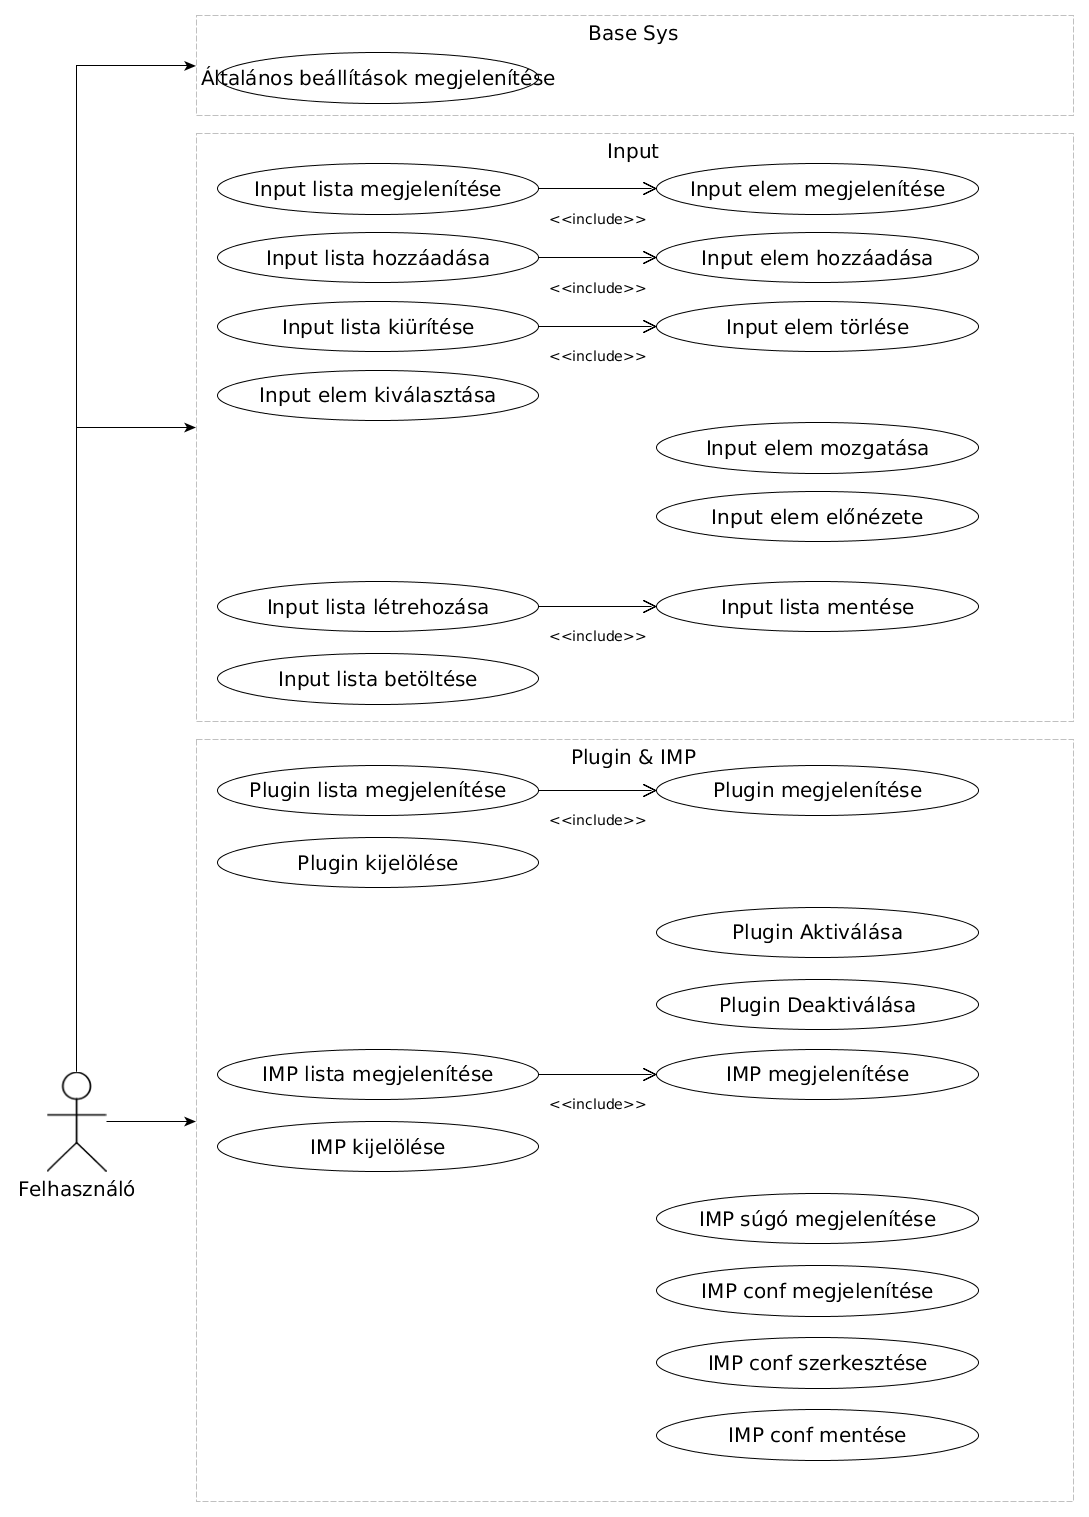
\includegraphics[width=\textwidth]{usecase_part_1.png}
  \caption{A BIMG teljes usecase diagrammja (1. rész) }
  \label{fig:bimg_usecase_schema_part_1}
\end{figure}
\begin{figure}[h]
  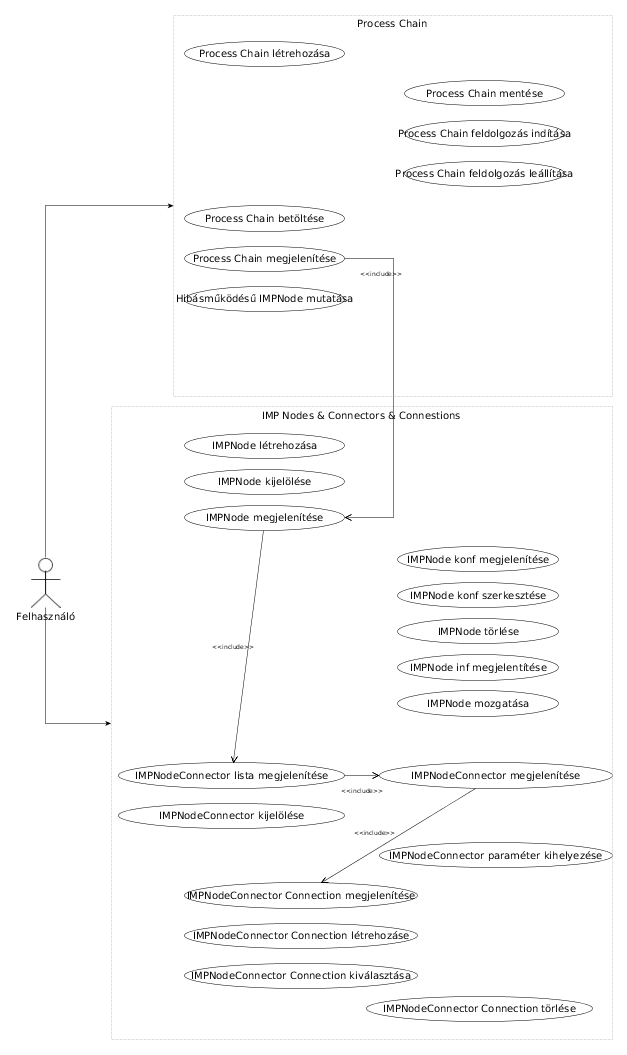
\includegraphics[width=\textwidth]{usecase_part_2.png}
  \caption{A BIMG teljes usecase diagrammja (2. rész) }
  \label{fig:bimg_usecase_schema_part_2}
\end{figure}

\subsection{CD melléklet}
A szakdolgozat CD mellékletének könyvtárszerkezete:

% itt a csel a [], amivel nem rak ki pontokat a latex
\begin{itemize}
    \item[] /VargaMarcell-DVLKHU-szakdolgozat.pdf
    \item[] /szakdolgozat-forraskod
    \begin{itemize}
        \item[] /diagramok
%        \item[] /kepek
%        \item[] /wireframek
        \item[] /szakdolgozat.tex
    \end{itemize}
    
    \item[] /rendszer-forraskod
    \begin{itemize}
 %       \item[] /app
        \item[] /src
        \begin{itemize}
  %          \item[] /google-api-php-client
            \item[] /Szakdolgozat
   %         \begin{itemize}
    %            \item[] FelhasznaloBundle
     %           \item[] JegyzokonyvBundle
      %          \item[] SzakdolgozatBundle
       %         \item[] UlesBundle
%            \end{itemize}
        \end{itemize}
        
%        \item[] /uploads
%        \item[] /web
    \end{itemize}
    
    \item[] /internetes-hivatkozasok
    \begin{itemize}
        \item[] /1\_osszehasonlitas
        \item[] /2\_kovetelmenyanalizis
    \end{itemize}
\end{itemize}

\end{document}